\chapter{Strategy模式}
\section{策略模式的概念}
\subsection{策略模式的定义}
策略(Strategy)模式的定义:该模式定义了一系列算法,并将每个算法封装起来,使它们可以相互替换,且算法的变化不会影响使用算法的客户。策略模式属于对象行为模式,它通过对算法进行封装,把使用算法的责任和算法的实现分割开来,并委派给不同的对象对这些算法进行管理。
\par 策略模式是准备一组算法,并将这组算法封装到一系列的策略类里面,作为一个抽象策略类的子类。策略模式的重心不是如何实现算法,而是如何组织这些算法,从而让程序结构更加灵活,具有更好的维护性和扩展性。
\subsection{优点}
\begin{enumerate}
	\item 多重条件语句不易维护,而使用策略模式可以避免使用多重条件语句;
	\item 策略模式提供了一系列的可供重用的算法族,恰当使用继承可以把算法族的公共代码转移到父类里面,从而避免重复的代码;
	\item 策略模式可以提供相同行为的不同实现,客户可以根据不同时间或空间要求选择不同的;
	\item 策略模式提供了对开闭原则的完美支持,可以在不修改原代码的情况下,灵活增加新算法;
	\item 策略模式把算法的使用放到环境类中,而算法的实现移到具体策略类中,实现了二者的分离。
\end{enumerate}
\subsection{缺点}
\begin{enumerate}
	\item 客户端必须理解所有策略算法的区别,以便适时选择恰当的算法类;
	\item 策略模式造成很多的策略类。
\end{enumerate}
\subsection{应用场景}
\begin{enumerate}
	\item 一个系统需要动态地在几种算法中选择一种时,可将每个算法封装到策略类中;
	\item 一个类定义了多种行为,并且这些行为在这个类的操作中以多个条件语句的形式出现,可将每个条件分支移入它们各自的策略类中以代替这些条件语句;
	\item 系统中各算法彼此完全独立,且要求对客户隐藏具体算法的实现细节时;
	\item 系统要求使用算法的客户不应该知道其操作的数据时,可使用策略模式来隐藏与算法相关的数据结构;
	\item 多个类只区别在表现行为不同,可以使用策略模式,在运行时动态选择具体要执行的行为。
\end{enumerate}
\subsection{角色}
\begin{enumerate}
	\item Strategy策略:负责实现策略所需接口API;
	\item ConcreteStrategy具体的策略:实现具体的策略;
	\item Context上下文:负责使用Strategy,保存了具体策略实例,并使用它。
\end{enumerate}
\section{策略模式实现——例一}
\begin{table}
	\begin{tabular}{|l|l|}
		\hline
		名字&说明\\
		\hline
		Hand&表示猜拳中的“手势”的类\\
		\hline
		Strategy&表示猜拳中的策略的类\\
		\hline
		WinningStrategy&表示“如果这局获胜,下一局也出一样的手势”这一策略的类\\
		\hline
		ProbStrategy&表示“根据上一局手势计算出下一局手势从之前结果计算下一局各种拳概率”\\
		\hline
		Player&表示进行猜拳游戏的选手的类\\
		\hline
		Main&测试程序的类\\
		\hline
	\end{tabular}
\end{table}
\begin{lstlisting}
public class Hand {
	public static final int HANDVALUE_GUU = 0;//代表石头
	public static final int HANDVALUE_CHO = 1;//代表剪刀
	public static final int HANDVALUE_PAA = 2;//代表步

	public static final Hand[] hand = {
		new Hand(HANDVALUE_GUU),
		new Hand(HANDVALUE_CHO),
		new Hand(HANDVALUE_PAA)
	};
	
	private static final String[] name = {
		"石头", "剪刀", "布"
	};
	private int handValue;//猜拳中出的值
	
	private Hand(int handValue) {
		this.handValue = handValue;
	}
	
	public static Hand getHand(int handValue) {
		return hand[handValue];
	}
	
	//判断是否强于对方
	public boolean isStrongerThan(Hand hand) {
		return fight(hand) == 1;
	}
	
	//判断是否弱于对方
	public boolean isWeakerThan(Hand hand) {
		return fight(hand) == -1;
	}
	
	private int fight(Hand hand) {
		if (this == hand) {
			return 0;
		} else if ((this.handValue + 1) % 3 == hand.handValue) {
			return 1;
		} else {
			return -1;
		}
	}
	public String toString() {
		return name[handValue];
	}
}
\end{lstlisting}
\begin{lstlisting}
public interface Strategy {
	Hand nextHand();
	
	//根据上一局输赢进行学习
	void study(boolean win);
}
\end{lstlisting}
\begin{lstlisting}
public class WinningStrategy implements Strategy {
	//如果上一局获胜,就和上一局出相同的
	//如果上一局失败,随机出
	//随机值,决定怎么出
	private Random random;
	//上一局的结果
	private boolean won = false;
	//上一局的手势
	private Hand prevHand;
	
	public WinningStrategy(int seed) {
		this.random = new Random(seed);
	}
	public Hand nextHand() {
		if (!won) {
			prevHand = Hand.getHand(random.nextInt(3));
		}
		return prevHand;
	}
	public void study(boolean win) {
		won = win;
	}
}
\end{lstlisting}
\begin{lstlisting}
public class ProbStrategy implements Strategy {
	//根据之前的猜拳结果概率决定
	
	private Random random;
	private int prevHandValue = 0;
	private int currentHandValue = 0;
	
	//history[上一局出的手势][这一局可能出的手势] 代表胜利的次数
	private int[][] history = {
		{1, 1, 1},
		{1, 1, 1},
		{1, 1, 1},
	};
	
	public ProbStrategy(int seed) {
		random = new Random(seed);
	}
	public Hand nextHand() {
		int bet = random.nextInt(getSum(currentHandValue));
		int handValue = 0;
		if (bet < history[currentHandValue][0]) {
			handValue = 0;
		} else if (bet < history[currentHandValue][1]) {
			handValue = 1;
		} else {
			handValue = 2;
		}
		prevHandValue = currentHandValue;
		currentHandValue = handValue;
		return Hand.getHand(handValue);
	}
	
	private int getSum(int hv) {
		int sum = 0;
		for (int i = 0; i < 3; i++) {
			sum += history[hv][i];
		}
		return sum;
	}
	public void study(boolean win) {
		if (win) {
			history[prevHandValue][currentHandValue]++;
		} else {
			history[prevHandValue][(currentHandValue + 1) % 3]++;
			history[prevHandValue][(currentHandValue + 2) % 3]++;
		}
	}
}
\end{lstlisting}
\begin{lstlisting}
public class Player {
	private String name;
	private Strategy strategy;
	private int winCount;
	private int loseCount;
	private int gameCount;
	public Player(String name, Strategy strategy) {
		this.name = name;
		this.strategy = strategy;
	}
	
	public Hand nextHand() {
		return strategy.nextHand();
	}
	
	public void win() {
		strategy.study(true);
		winCount++;
		gameCount++;
	}
	
	public void lose() {
		strategy.study(false);
		loseCount++;
		gameCount++;
	}
	
	public void even() {
		gameCount++;
	}
	
	public String toString() {
		return "Player{" +
		"name='" + name + '\'' +
		", winCount=" + winCount +
		", loseCount=" + loseCount +
		", gameCount=" + gameCount +
		'}';
	}
}
\end{lstlisting}
\begin{lstlisting}
public class Main {
	//生成两个选手,采取不同的策略
	public static void main(String[] args) {
		Scanner scanner = new Scanner(System.in);
		int seed1 = scanner.nextInt();
		int seed2 = scanner.nextInt();
		Player player1 = new Player("Taro", new WinningStrategy(seed1));
		Player player2 = new Player("Hana", new ProbStrategy(seed2));
		for (int i = 0; i < 10000; i++) {
			Hand nextHand1 = player1.nextHand();
			Hand nextHand2 = player2.nextHand();
			if (nextHand1.isStrongerThan(nextHand2)) {
				System.out.println("Winner: " + player1);
				player1.win();
				player2.lose();
			} else if (nextHand2.isStrongerThan(nextHand1)) {
				System.out.println("Winner: " + player2);
				player2.win();
				player1.lose();
			} else {
				System.out.println("Even...");
				player1.even();
				player2.even();
			}
		}
		System.out.println("Total result: ");
		System.out.println(player1.toString());
		System.out.println(player2.toString());
	}
}
\end{lstlisting}
\section{策略模式实现——例二}
\begin{figure}[!h]
	\centering
	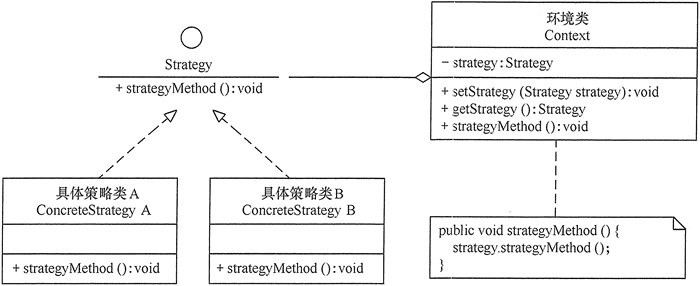
\includegraphics[width=0.8\textwidth]{image/10-1}
	\caption{策略模式的结构图}
\end{figure}
\begin{lstlisting}
//抽象策略类
interface Strategy {
	public void strategyMethod();    //策略方法
}

//具体策略类A
class ConcreteStrategyA implements Strategy {
	public void strategyMethod() {
		System.out.println("具体策略A的策略方法被访问!");
	}
}

//具体策略类B
class ConcreteStrategyB implements Strategy {
	public void strategyMethod() {
		System.out.println("具体策略B的策略方法被访问!");
	}
}
\end{lstlisting}
\begin{lstlisting}
//环境类
class Context {
	private Strategy strategy;
	
	public Strategy getStrategy() {
		return strategy;
	}
	
	public void setStrategy(Strategy strategy) {
		this.strategy = strategy;
	}
	
	public void strategyMethod() {
		strategy.strategyMethod();
	}
}
\end{lstlisting}
\begin{lstlisting}
public class StrategyPattern {
	public static void main(String[] args) {
		Context c = new Context();
		Strategy s = new ConcreteStrategyA();
		c.setStrategy(s);
		c.strategyMethod();
		System.out.println("-----------------");
		s = new ConcreteStrategyB();
		c.setStrategy(s);
		c.strategyMethod();
	}
}
\end{lstlisting}
\begin{lstlisting}
//output
具体策略A的策略方法被访问!
-----------------
具体策略B的策略方法被访问!
\end{lstlisting}
\section{策略模式扩展}
在一个使用策略模式的系统中,当存在的策略很多时,客户端管理所有策略算法将变得很复杂,如果在环境类中使用策略工厂模式来管理这些策略类将大大减少客户端的工作复杂度。
\begin{figure}[!h]
	\centering
	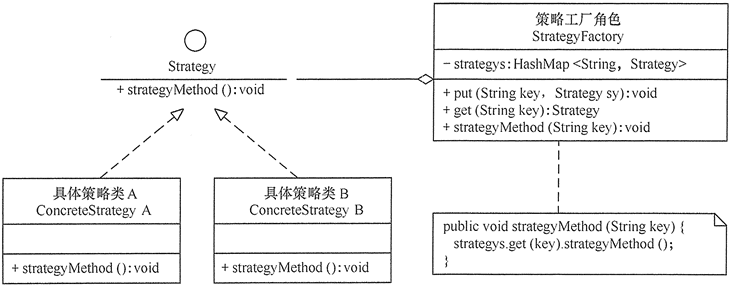
\includegraphics[width=0.8\textwidth]{image/10-2}
	\caption{策略工厂模式的结构图}
\end{figure}
\section{扩展思路}
\begin{enumerate}
	\item 为什么使用Strategy角色?使用委托这种弱关联可以方便的整体替换算法。
	\item 程序运行中可以切换策略。
\end{enumerate}
\section{相关模式}
\begin{enumerate}
	\item Flyweight模式会让多个地方共用ConcreteStrategy角色;
	\item 策略模式可以整体替换算法,抽象工厂可以整体替换工厂、零件、产品;
	\item 使用Strategy和State都可以替换被委托的对象,两者类之间关系很相似,但目的不同:
	\begin{itemize}
		\item Strategy:ConcreteStrategy角色是表示算法的类。可以替换被委托对象的类;
		\item State:ConcreteState是表示状态的类,每次状态变化时,被委托的类必定会被替换。
	\end{itemize}
\end{enumerate}